\documentclass[10pt, aspectratio=169]{beamer}
\usefonttheme{professionalfonts}
%\usetheme{CambridgeUS}
%
% Choose how your presentation looks.
%
% For more themes, color themes and font themes, see:
% http://deic.uab.es/~iblanes/beamer_gallery/index_by_theme.html
%
\mode<presentation>
{
  \usetheme{default}      % or try Darmstadt, Madrid, Warsaw, ...
  \usecolortheme{beaver} % or try albatross, beaver, crane, ...
  \usefonttheme{default}  % or try serif, structurebold, ...
  \setbeamertemplate{navigation symbols}{}
  \setbeamertemplate{caption}[numbered]
} 

\usepackage[english]{babel}
\usepackage[utf8x]{inputenc}
\usepackage{tikz}
\usepackage{pgfplots}
\usepackage{array}  % for table column M
\usepackage{makecell} % to break line within a cell
\usepackage{verbatim}
\usepackage{graphicx}
\usepackage{epstopdf}
\usepackage{amsfonts}
\usepackage{xcolor}
%\captionsetup{compatibility=false}
%\usepackage{dsfont}
\usepackage[absolute,overlay]{textpos}
\usetikzlibrary{calc}
\usetikzlibrary{pgfplots.fillbetween, backgrounds}
\usetikzlibrary{positioning}
\usetikzlibrary{arrows}
\usetikzlibrary{pgfplots.groupplots}
\usetikzlibrary{arrows.meta}
\usetikzlibrary{plotmarks}

\usepgfplotslibrary{groupplots}
\pgfplotsset{compat=newest} 
%\pgfplotsset{plot coordinates/math parser=false}

\usepackage{hyperref}
\hypersetup{
    colorlinks=true,
    linkcolor=blue,
    filecolor=magenta,      
    urlcolor=cyan,
}

%% 
\def\EXTERNALIZE{1} % for externalizing figures
\input{header.tex}

\title[EE 264]{Changing the Sampling Rate in DSP}
\author{Jose Krause Perin}
\institute{Stanford University}
\date{July 11, 2017}

\begin{document}

\begin{frame}
  \titlepage
\end{frame}

\begin{frame}{Last lecture}
\begin{itemize}
	\item Sampling a continuous-time signal results in replicas of the spectrum at multiples of the sampling frequency $\Omega_s$ (or $2\pi$ of the normalized frequency $\omega$)
	\item A band-limited signal has highest frequency $\Omega_N$ ($X_c(j\Omega) = 0, |\Omega| > \Omega_N$)
	\item If a band-limited signal is oversampled ($\Omega_s > 2\Omega_N$) there'll be gaps between the spectrum replicas
	\item If the signal is undersampled ($\Omega_s < 2\Omega_N$) the spectrum replicas will overlap resulting in aliasing distortion
	\item We can perfectly reconstruct a signal from its samples, provided that there is no aliasing and that we use the ideal lowpass filter as reconstruction filter
	\item In practice, we use different reconstruction filters, since the ideal lowpass filter is unfeasible.
	\item Oversampling relaxes the reconstruction filter specifications
	\item In theory, we can perform any LTI continuous-time filtering in discrete-time (in DSP), provided that there is no aliasing and that we use the ideal reconstruction filter
\end{itemize}
\end{frame}

%
\begin{frame}{Today's lecture} 

\begin{itemize}
	\item Downsampling and decimation
	\item Upsampling and interpolation
	\item Noninteger rate change
	\item Multi-rate processing
\end{itemize}
\end{frame}

%
\section{Downsampling and Decimation}
\begin{frame}{Downsampling}

Downsampling by an integer factor $M$ is equivalent to sampling the discrete-time signal $x[n]$ with sampling period $M$. 

\begin{center}
	\resizebox{0.6\linewidth}{!}{\input{figs/downsampling_block.tex}}
\end{center}

To understand what happens in the frequency domain, we can think that we're sampling the original continuous-time signal $x_c(t)$ with sampling period $T_d = MT$:
\begin{equation*}
x_d[n] = x[Mn] = x_c(nMT)
\end{equation*}

\end{frame}
	
%	
\begin{frame}{Downsampling: frequency domain interpretation}
\fontsize{9pt}{7.2}\selectfont
%\vspace{-1cm}
Sampling $x_c(t)$ with sampling period $T_d = MT$ results in
\begin{align*}
	X_d(e^{j\omega}) &= \frac{1}{T_d}\sum_{k = -\infty}^{\infty} X_c\Big[j\Big(\frac{\omega}{T_d} - \frac{2\pi k}{T_d}\Big)\Big] \tag{spectrum replicas appear with period $\Omega_s = 2\pi/T_d$} \\
	&= \frac{1}{MT}\sum_{k = -\infty}^{\infty} X_c\Big[j\Big(\frac{\omega}{MT} - \frac{2\pi k}{MT}\Big)\Big] \tag{$T_d = MT$} \\
	&= \frac{1}{MT}\sum_{m = 0}^{M-1}\sum_{l = -\infty}^{\infty} X_c\Big(j\Big(\frac{\omega}{MT} - \frac{2\pi l}{T} - \frac{2\pi m}{MT}\Big)\Big) \tag{change of variables: $k = m + lM$} \\
	&= \frac{1}{M}\sum_{m = 0}^{M-1}\tikz[baseline]{\node[fill=blue!20,anchor=base] (t1) {$\displaystyle\frac{1}{T}\sum_{l = -\infty}^{\infty} X_c\Big(j\Big(\frac{\omega - 2\pi m}{MT} - \frac{2\pi l}{T}\Big)\Big)$};} \tag{rearranging} \\
	&= \frac{1}{M}\sum_{m = 0}^{M-1} X(e^{j\omega^{\prime}})\Big|_{\omega^{\prime} = \frac{\omega-2\pi m}{M}} \tag{$\tikz[baseline]{\node[fill=blue!20,anchor=base] {$^{~}$};}$ is equivalent to $X(e^{j\omega^{\prime}})$ for $\omega^{\prime} = \frac{\omega-2\pi m}{M}$}
\end{align*}

\textbf{Conclusion:} $X(e^{j\omega})$ is stretched by a factor of $M$ ($\omega/M$), and there will be replicas of the spectrum with period $2\pi/M$.
\end{frame}

%
\begin{frame}{Downsampling: frequency domain interpretation}
Example of downsampling with $M = 2$ i.e., $T_d = 2T$.

\textbf{Impulse sampling interpretation:}
\begin{center}
	\resizebox{0.65\linewidth}{!}{\input{figs/downsampling_freq_domain_ct.tex}}
\end{center}
\onslide<3|handout:1>{After downsampling spectrum replicas appear with period $2\pi/T_d$}
\end{frame}

%
\begin{frame}{Downsampling: frequency domain interpretation}
Same example of downsampling with $M = 2$ i.e., $T_d = 2T$.

\textbf{Discrete-time interpretation:}
\begin{center}
	\resizebox{0.65\linewidth}{!}{\input{figs/downsampling_freq_domain.tex}}
\end{center}
\onslide<3|handout:1>{To obtain the spectrum we discrete time, we just need to use the change of variables $\omega = \Omega T$ and $\omega = \Omega T_d$}
\end{frame}

%
\begin{frame}{Downsampling: frequency domain interpretation}
Downsampling may lead to spectrum overlapping (\textbf{aliasing distortion}).

Example of downsampling with $M = 3$ i.e., $T_d = 3T$.
\begin{center}
	\resizebox{0.65\linewidth}{!}{\input{figs/downsampling_freq_domain_aliasing.tex}}
\end{center}
\end{frame}

%
\begin{frame}{Decimation}
Similarly to sampling, it is common to employ an \textbf{anti-aliasing filter} before downsampling in order to minimize aliasing. 

Pre-filtering followed by downsampling is called \textbf{decimation}.

\begin{center}
	\resizebox{0.85\linewidth}{!}{\input{figs/decimation_block.tex}}
\end{center}
\vspace{-0.5cm}
\begin{align}
x[n] \Longleftrightarrow & X(e^{j\Omega T}) = \frac{1}{T}\sum_{k = -\infty}^\infty X_c\Big(j\Big(\Omega - \frac{2\pi k}{T}\Big)\Big) \tag{from sampling} \\
\tilde{x}[n] \Longleftrightarrow & \tilde{X}(e^{j\Omega T}) = H(e^{j\Omega T})X(e^{j\Omega T}) \tag{LTI output} \\
x_d[n] = \tilde{x}[nM] \Longleftrightarrow & \frac{1}{M}\sum_{m = 0}^{M-1} \tilde{X}(e^{j(\Omega T - 2\pi T)/M}) \tag{downsampling by $M$}
\end{align}

\end{frame}

%
\begin{frame}{Decimation: frequency domain interpretation}
Decimation with $M = 3$ i.e., $T_d = 3T$.
\begin{center}
	\resizebox{0.6\linewidth}{!}{\input{figs/decimation_freq_domain.tex}}
\end{center}
\onslide<4|handout:1>{Now the spectrum replicas do not overlap after downsampling by 3.}
\end{frame}

%
\section{Upsampling and Interpolation}
\begin{frame}{Interpolation}
Interpolation is used to increase the sampling rate by an integer factor $L$.

\begin{center}
	\resizebox{0.6\linewidth}{!}{\input{figs/upsampling_block.tex}}
\end{center}
\vspace{-0.2cm}
\begin{equation*}
x_e[n] = \begin{cases}
x[n/L], & 0, \pm L, \pm 2L, \ldots \\
0, & \text{otherwise}
\end{cases}\tag{after upsampling}
\end{equation*}

\pause
In the frequency domain:
\begin{align*}
X_e(e^{j\omega}) &= \sum_{n = -\infty}^{\infty} x_e[n]e^{-j\omega n} \tag{definition of DTFT} \\
&= \sum_{n = 0, \pm L, \ldots} x[n/L]e^{-j\omega n} \tag{from $x_e[n]$ equation above} \\
&= \sum_{k = -\infty}^{\infty} x[k]e^{-j\omega kL} \tag{change of variable: $k = n/L$} \\
&= X(e^{j\omega L}) \tag{from DTFT equation with $\omega L$}
\end{align*}
\end{frame}

%
\begin{frame}{Interpolation: frequency domain interpretation}
Example of interpolation with $L = 2$
\begin{center}
	\resizebox{0.55\linewidth}{!}{\input{figs/upsampling_freq_domain.tex}}
\end{center}
\end{frame}

%
\begin{frame}{Practical interpolation filters}
\begin{itemize}
	\item Similarly to what we saw in reconstruction (D-to-C), the ideal lowpass filter is not practical. Hence, we must use practical interpolation filters such as ZOH, linear interpolator, or cubic spline.
	\item \textbf{One important difference:} The interpolation filter used in reconstruction to convert from discrete-time to continuous-time was an analog filter (a continuous-time filter). The interpolation filter used for upsampling is realized in discrete-time (in DSP). Therefore, we have more flexibility.
\end{itemize}
\end{frame}

%
\begin{frame}{Example of interpolation}
\begin{itemize}
	\item The original signal has maximum frequency $\Omega_N = 1$ rad/s. 
	\item From the Nyquist-Shannon theorem, we need $\Omega_s > 2\Omega_N$ in order to be able to achieve perfect reconstruction. Or equivalently, $T < \pi$ s. 
	\item Sampling period is $T = \pi$
\end{itemize}

\begin{center}
	\resizebox{0.6\linewidth}{!}{\input{figs/interpolation_example.tex}}
\end{center}
\onslide<4|handout:1> {Truncated sinc filter had 11 coefficients, while ZOH had 2 and linear interpolator had 3.}
\end{frame}

%
\begin{frame}{Example of interpolation}
Same example as before, but now sampling period is $T = 0.4\pi$.

\begin{center}
	\resizebox{0.7\linewidth}{!}{\input{figs/interpolation_example_oversampled.tex}}
\end{center}
\onslide<4|handout:1> {Truncated sinc filter had 11 coefficients, while ZOH had 2 and linear interpolator had 3.}
\end{frame}

%
\begin{frame}<beamer:1|handout:1>
%\fontsize{9pt}{7.2}\selectfont
\begin{itemize}
	\item In the first example the continuous-time signal was sampled at the Nyquist rate, whereas in the second example the continuous-time signal was oversampled by 2.5.
	\item In both cases, we upsample by a factor of 2 and use practical reconstruction filters: ZOH, a linear interpolator, and a truncated sinc with 11 samples.
	\item The ZOH filter only has two coefficients, the linear interpolator has three coefficents, and the truncated sinc has 11 coefficients.
	\item Although we use the same filters in both examples, the interpolated sequences are much closer to the original continuous-time signal in the second example. This illustrates how oversampling can help the interpolation filters.
	\item In these examples, the linear interpolator offers that best performance vs complexity trade-off, as it achieves performance close to the truncated sinc, but only uses 3 samples.
	\item Even with high oversampling, we see that the truncated sinc filter didn't achieve perfect reconstruction. This is a consequence of the \textbf{Gibbs phenomenon}, discussed in lecture 1. Recall that a truncated sinc will produce a DTFT that is different from the ideal lowpass filter. Specifically, the DTFT of the truncated sequence will have oscillations, which will affect the signal and will not suppress the spectrum replicas centered at multiples of $2\pi$. Using an even larger sequence (sinc with more samples) would not help much, since the ripples would only become more rapid, but their amplitude would not decrease.
\end{itemize}
\end{frame}


\begin{frame}{In Matlab}

Sampled signal with period $T$\\
\texttt{>> T = 0.5*pi} \\
\texttt{>> t = -20:T:20} \\
\texttt{>> x = cos(t/2) - sin(t) + cos(t/2-pi/4) - sin(t/4-deg2rad(154)); {\color{matlabcomment} \% Sampled signal}} \\ 

Upsample\\
\texttt{>> xu = upsample(x, L)  {\color{matlabcomment} \% Upsample}} \\ 

Interpolation filters \\
\texttt{>> hZOH = [1 1]  {\color{matlabcomment} \% ZOH}} \\ 
\texttt{>> hlin = [1/2 1 1/2] {\color{matlabcomment} \% Linear interpolator}} \\ 
\texttt{>> hsinc = sinc(-(5:5)/2) {\color{matlabcomment} \% truncated sinc with 11 samples}} \\

Interpolate \\
\texttt{>> yzoh = filter(hZOH, 1, xu)} \\
\texttt{>> ylin = filter(hlin, 1, xu)} \\
\texttt{>> ysinc = filter(hsinc, 1, xu)} \\
\texttt{{\color{matlabcomment} \% since these filters are FIR we could also have used the conv command}}
~\\

Before plotting we need to remove the group delay introduced by the filters (more on this next week)
\end{frame}

% 
\section{Non-Integer Rate Change}
\begin{frame}{Interpolation/Decimation by a non-integer factor}
\begin{itemize}
	\item We have seen how to increase the sampling period by an integer factor $M$ and how to decrease the sampling period by an integer factor $L$
	\item By cascading interpolation and decimation we can change the sampling period by a non-integer factor $M/L$.
\end{itemize}

\begin{block}{Cascading interpolation and decimation}
\begin{center}
	\resizebox{0.85\linewidth}{!}{\input{figs/non-integer_rate_change_diagram.tex}}
\end{center}
\end{block}
\vspace{-0.5cm}
\onslide<2|handout:1>{
\begin{block}{Equivalent diagram}
\begin{center}
	\resizebox{0.55\linewidth}{!}{\input{figs/non-integer_rate_change_equivalent_diagram.tex}}
\end{center}
\end{block}
}
\end{frame}


\begin{frame}{Example}
	\only<1-3|handout:1>{
	\begin{itemize}
		\item Let's combine the examples we saw earlier with $L = 2$ and $M = 3$. Recall that with $M = 3$, there would be aliasing if we didn't use the anti-aliasing filter. 
		\item The filter cutoff is $\min(\pi/2, \pi/3) = \pi/3$.
	\end{itemize}
	}
	\only<4-|handout:2>{
		continuing...
	}
	\begin{center}
		\resizebox{0.65\linewidth}{!}{\input{figs/non-integer_rate_change_freq_domain.tex}}
	\end{center}
	\only<5-|handout:2>{
		The resulting signal has sampling period $MT/L = 3T/2$. Note that aliasing was prevented by selecting the cutoff frequency $\min(\pi/2, \pi/3) = \pi/3$.
	}
\end{frame}

% 
\section{Multi-rate processing}
\begin{frame}{Multirate processing}
	In practice, it is common to have parts of the system operating at one sampling rate and other parts operating at a different sampling rate.
	\begin{itemize}
		\item Interchanging filtering and downsampling
		\item Interchanging filtering and upsampling
		\item Multi-stage decimation
		\item Multi-stage interpolation
		\item Polyphase decomposition
	\end{itemize}

\end{frame}

\begin{frame}{Interchanging filtering and downsampling}
	These two systems are equivalent i.e., $y_1[n] = y_2[n]$
	\begin{center}
		\resizebox{0.6\linewidth}{!}{\input{figs/interchange_filter_downsampling.tex}}
	\end{center}	

	To move the filter before downsampling by $M$, we must stretch its frequency response by a factor of $M$: $H(z^M) \xrightarrow{z = e^{j\omega}} H(e^{j\omega M})$.
\end{frame}

\begin{frame}
	\textit{Proof:}
	
	Staring with the second system: $X_2(e^{j\omega}) = H(e^{j\omega M})X(e^{j\omega})$. Now we can apply the equation for downsampling to obtain $Y_2(e^{j\omega})$
	\begin{align*}
	Y_2(e^{j\omega}) &= \frac{1}{M}\sum_{m= 0}^{M-1} X_2(e^{j(\omega/M - 2\pi m)}) \\
	&=\frac{1}{M}\sum_{m= 0}^{M-1} X(e^{j(\omega/M - 2\pi m)})H(e^{j(\omega - 2\pi m)}) \\
	&=H(e^{j\omega})\frac{1}{M}\sum_{m= 0}^{M-1} X(e^{j(\omega/M - 2\pi m)}) \tag{periodicity of the DTFT $\implies H(e^{j(\omega - 2\pi m)}) = H(e^{j\omega})$} \\
	&=H(e^{j\omega})\tikz[baseline]{\node[fill=blue!20,anchor=base] {$\displaystyle\frac{1}{M}\sum_{m= 0}^{M-1} X(e^{j(\omega/M - 2\pi m)})$};} \\
	&=H(e^{j\omega})\tikz[baseline]{\node[fill=blue!20,anchor=base] {$X_1(e^{j\omega})$};} = Y_1(e^{j\omega})
	\end{align*}
\end{frame}

\begin{frame}
\textbf{Comments on stability:}

Note that if $H(z)$ is a rational $z$-transform with poles $\{p_1, p_2, \ldots, p_N\}$ and zeros $\{z_1, z_2, \ldots, z_R\}$:
\begin{equation*}
H(z) = \frac{b_0}{a_0}z^{N-R}\frac{(z-z_1)(z-z_2)\ldots(z-z_R)}{(z-p_1)(z-p_2)\ldots(z-p_N)}
\end{equation*}
Then $H(z^M)$ will be
\begin{equation*}
H(z^M) = \frac{b_0}{a_0}z^{M(N-R)}\frac{(z^M-z_1)(z^M-z_2)\ldots(z^M-z_R)}{(z^M-p_1)(z^M-p_2)\ldots(z^M-p_N)},
\end{equation*}
with poles $\{\sqrt[M]{p_1}, \sqrt[M]{p_N}, \ldots, \sqrt[M]{p_N}\}$, and zeros $\{\sqrt[M]{z_1}, \sqrt[M]{z_N}, \ldots, \sqrt[M]{z_R}\}$.
 
If $H(z)$ is stable and \textbf{causal}, the poles of $H(z^M)$ will lie \underline{inside the unit circle}, and therefore $H(z^M)$ will also be stable.

Similarly, if $H(z)$ is \textbf{anti-causal} and stable, the poles of $H(z^M)$ will lie \underline{outside the unit circle}, and therefore $H(z^M)$ will also be stable.

\end{frame}


\begin{frame}{Interchanging filtering and interpolation}
	These two systems are equivalent i.e., $y_1[n] = y_2[n]$
	\begin{center}
		\resizebox{0.5\linewidth}{!}{\input{figs/interchange_filter_interpolation.tex}}
	\end{center}	
	\textit{Proof:}
	
	Top diagram:
	\begin{align*}
	Y_1(e^{j\omega}) = X_1(e^{j\omega L}) = X(e^{j\omega L})H(e^{j\omega L}) 
	\end{align*}
	
	Bottom diagram:
	\begin{align*}
	Y_2(e^{j\omega}) = X_2(e^{j\omega})H(e^{j\omega L}) = X(e^{j\omega L})H(e^{j\omega L}) 
	\end{align*}
\end{frame}

\begin{frame}{Multi-stage decimation}
	Suppose we want to decimate by a factor $M = 20$. The cutoff frequency of the lowpass filter would be $\pi/20$. 
	\begin{equation*}
	\text{Sharp  filter} \implies \text{long impulse response} \implies \begin{array}{c}
	\text{higher complexity} \\
	\text{higher cost} \\
	\text{higher power consumption} 
	\end{array}
	\end{equation*}
	
	\pause
	It's more efficient to use several decimation stages
	\begin{center}
		\resizebox{0.45\linewidth}{!}{\input{figs/multistage_decimation_block.tex}}
	\end{center}	
	\pause
	
	Interchanging filter and downsampling results in the equivalent system:
	
	\begin{center}
	\resizebox{0.45\linewidth}{!}{
		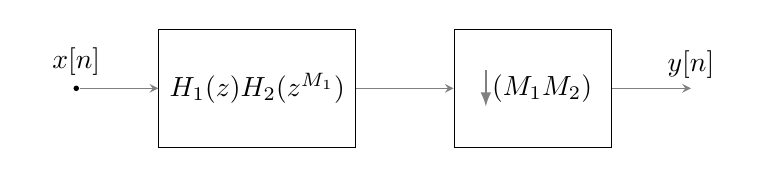
\begin{tikzpicture}[->, >=stealth, shorten >= 0pt, draw=black!50, node distance=3.5cm, font=\sffamily]
			\tikzstyle{node}=[circle,fill=black,minimum size=2pt,inner sep=0pt]
			\tikzstyle{block}=[draw=black,rectangle,fill=none,minimum size=1.5cm, inner sep=0pt]
			
			\node[node] (xc) {};
			\node[block, right=1cm of xc, text width = 2.5cm, align= center] (AA) {$H_1(z)H_2(z^{M_1})$};
			\node[block, right of=AA, text width = 2cm, align= center] (DSP) {$~~(M_1M_2)$};
			\draw[-latex, shorten >= 15pt, shorten <= 15pt, line width=0.75pt] ($(DSP.north)-(17pt, 0)$) -- ($(DSP.south)-(17pt, 0)$) {};
			\coordinate (yc) at ($(DSP.east)+(1cm, 0)$) {};
						
			\path (xc) edge (AA);
			\path (AA) edge (DSP);
			\path (DSP) edge (yc);
			
			\node[above = 0mm of xc, text width = 1cm, align=center] {$x[n]$};
			\node[above = 0mm of yc, text width = 1cm, align=center] {$y[n]$};
		\end{tikzpicture}
	}
	\end{center}
	
	\begin{itemize}
		\item The equivalent downsampling factor is $M = M_1M_2$.
		\item Design $H_1(z)$ and $H_2(z)$ so that $H_1(z)H_2(z^{M_1})$ has the desired frequency response. 
	\end{itemize}	
\end{frame}

\begin{frame}{Multi-stage interpolation}
	The same rationale applies to interpolation
	\begin{center}
		\resizebox{0.6\linewidth}{!}{\input{figs/multistage_interpolation_block.tex}}
	\end{center}	
	Interchanging filter and downsampling results in the equivalent system:
	
	\begin{center}
		\resizebox{0.6\linewidth}{!}{
			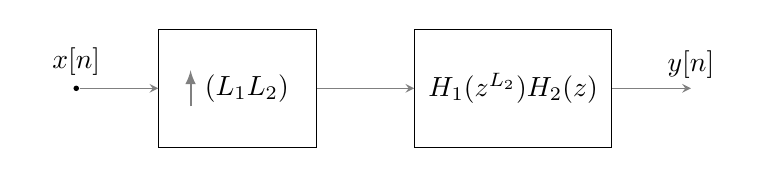
\begin{tikzpicture}[->, >=stealth, shorten >= 0pt, draw=black!50, node distance=3.5cm, font=\sffamily]
			\tikzstyle{node}=[circle,fill=black,minimum size=2pt,inner sep=0pt]
			\tikzstyle{block}=[draw=black,rectangle,fill=none,minimum size=1.5cm, inner sep=0pt]
			
			\node[node] (xc) {};
			\node[block, right=1cm of xc, text width = 2cm, align= center] (DSP) {$~~(L_1L_2)$};
			\draw[-latex, shorten >= 15pt, shorten <= 15pt, line width=0.75pt] ($(DSP.south)-(17pt, 0)$) -- ($(DSP.north)-(17pt, 0)$) {};
			\node[block, right of=DSP, text width = 2.5cm, align= center] (AA) {$H_1(z^{L_2})H_2(z)$};

			\coordinate (yc) at ($(AA.east)+(1cm, 0)$) {};
			
			\path (xc) edge (DSP);
			\path (DSP) edge (AA);
			\path (AA) edge (yc);
			
			\node[above = 0mm of xc, text width = 1cm, align=center] {$x[n]$};
			\node[above = 0mm of yc, text width = 1cm, align=center] {$y[n]$};
			\end{tikzpicture}
		}
	\end{center}
	
	\begin{itemize}
		\item The equivalent upsampling factor is $L = L_1L_2$.
		\item Design $H_1(z)$ and $H_2(z)$ so that $H_1(z^{L_2})H_2(z)$ has the desired frequency response. 
	\end{itemize}	
\end{frame}

\begin{frame}{Polyphase decomposition}
	What if the filter is placed before downsampling?
	\begin{center}
		\resizebox{0.6\linewidth}{!}{\input{figs/filter_downsampling.tex}}
	\end{center}
	\begin{itemize}
		\item To interchange filter and downsampling in this case, we'd need to express $H(z)$ as some $G(z^M)$. Generally not easy.
		\item \textbf{Practical problem:} this implementation wastes computation. All samples of the output of $H(z)$ are calculated, but only 1 out of $M$ is used after downsampling. 
		\item If $H(z)$ is FIR of length $N$, there are $N$ multiplications per sample. Downsampling by $M$ discards $M-1$ samples every $M$ samples.
	\end{itemize}
\end{frame}

\begin{frame}{Polyphase decomposition}
	We can decompose any given sequence $h[n]$ into $M$ subsequences such that
	\begin{equation*}
	h_k[n] = \begin{cases}
	h[n+k], & n~\text{integer multiple of } M \\
	0, & \text{otherwise}
	\end{cases}, k = 0, 1, \ldots, M-1
	\end{equation*}
	
	It follows that
	\begin{equation*}
	h[n] = \sum_{k = 0}^{M-1} h_k[n-k] \Longleftrightarrow H(z) = \sum_{k = 0}^{M-1} H_k(z)z^{-k}
	\end{equation*}
\end{frame}	
	
\begin{frame}{Polyphase decomposition}	
	Example of decomposition with $M = 2$
	
	\begin{center}
	\resizebox{0.6\linewidth}{!}{\input{figs/polyphase_decomposition_time_domain.tex}}
\end{center}	
\end{frame}


\begin{frame}{Polyphase decomposition}
	We can downsample $h_k[n]$ in order to discard the zero samples
	\begin{equation*}
	e_k[n] = h_k[Mn] \Longleftrightarrow E_k(z^M) = H_k(z) \tag{upsamling by M}
	\end{equation*}

	The subsequences $e_k[n]$ are called the \textbf{polyphase components} of $h[n]$
	\begin{center}
		\resizebox{0.5\linewidth}{!}{\input{figs/polyphase_decomposition_e_time_domain.tex}}
	\end{center}	
\end{frame}

\begin{frame}{Polyphase decomposition}
	How to recover $h[n]$ from $e_0[n], \ldots, e_{M-1}[n]$?
	
	\begin{enumerate}
		\item Upsample $e_k[n]$ by $M$, and we're back with $h_k[n]$
		\item Delay by $k$ and add
	\end{enumerate}

	In terms of the $z$-transform:
	\begin{equation*}
	H(z) = \sum_{k=0}^{M-1} E_k(z^M)z^{-k}
	\end{equation*}
	
	\begin{center}
		\resizebox{0.6\linewidth}{!}{\input{figs/polyphase_decomposition_diagram.tex}}
	\end{center}
\end{frame}

\begin{frame}{Polyphase decimation}
	Back to the original problem: how to interchange filter and downsampling?
	\begin{center}
		\resizebox{0.5\linewidth}{!}{\input{figs/filter_downsampling.tex}}
	\end{center}
	Using the polyphase decomposition of $H(z)$
	\begin{center}
		\def\DOWN{1}
		\resizebox{0.8\linewidth}{!}{\input{figs/polyphase_decomposition_diagram.tex}}
	\end{center}
\end{frame}

%
\begin{frame}{Polyphase decimation}
	First interchange sum and downsampling:
 	\begin{center}
	 	\resizebox{0.9\linewidth}{!}{\input{figs/polyphase_decomposition_diagram2.tex}}
 	\end{center}
\end{frame}

%
\begin{frame}{Polyphase decimation}
	Now it is easy to interchange $E_k(\tikz[baseline]{\node[fill=blue!20,anchor=base] {$z^M$};})$ with downsampling resulting in the filters $E_k(\tikz[baseline]{\node[fill=blue!20,anchor=base] {$z$};})$
	\begin{center}
		\resizebox{0.9\linewidth}{!}{\input{figs/polyphase_decomposition_diagram3.tex}}
	\end{center}
\textbf{Computation:} Each polyphase filter $E_k(z)$ requires $N/M$ multiplications, which are realized at the lower rate (higher sampling period) $TM$.

Similarly for polyphase interpolation (Textbook section 4.7.5)

\end{frame}

%
\begin{frame}{Summary}
\begin{itemize}
	\item Downsampling by an integer factor $M$ stretches the discrete-time spectrum by a factor $M$ and causes replicas of the spectrum to appear at $2\pi/M$. The amplitude of the spectrum is attenuated by $M$
	\item It's often easier to think of downsampling as sampling the original continuous-time signal with a sampling period $T_d = MT$
	\item Anti-aliasing filtering followed by downsampling is called decimation
	\item Upsampling by an integer factor $L$ compresses the discrete-time spectrum by a factor $L$. The interpolation filter is assumed to have gain $L$, so the spectrum amplitude is scaled by $L$
	\item We can achieve non-integer sampling rate changes by cascading interpolation and decimation stages
	\item For large downsampling/uspsampling factors, it's generally more efficient to realized multistage decimation/interpolation
	\item Polyphase decomposition allows efficient implementation of filtering followed by downsampling and upsampling followed by filtering.
\end{itemize}
\end{frame}

\end{document}
